

%% La classe stageM2R s'appuie sur la classe memoir, plus d'information sur le paquet: http://www.ctan.org/pkg/memoir
%% option possible de la classe stageM2R
% utf8  -> encodage du texte UTF8 (défaut: Latin1)
% final -> mode rapport de stage final (défaut: mode étude bibliographique)
% private -> indique une soutenance privée (défaut: soutenance publique)
\documentclass[utf8]{stageM2R} %-> etude bibliographique
%\documentclass[utf8,final]{stageM2R} %-> rapport final

%%%%%%%%%%%%%%%%%%%%%%%%%%%%
%%% Déclaration du stage %%%
%%%%%%%%%%%%%%%%%%%%%%%%%%%%

\usepackage{graphicx}
\usepackage{color}
\usepackage{listings}
\usepackage{bussproofs}
\usepackage{textcomp}

%% auteur
\author{Jimmy Lopez}
%% encadrants
\supervisors{David Delahaye\\Christophe Dony\\Chouki Tibermacine}
%% lieu du stage (Optionnel)
\location{LIRMM UM5506 - CNRS, Université de Montpellier}
%% titre du stage
\title{Formalisation de la sémantique d’un langage à composants} 
%% parcours du master
\track{AIGLE}  
%% date de soutenance (Optionnel)
\date{\today} 
%% version du rapport (Optionnel)
\version{1}
%% Résumé en francais
%%\abstractfr{
%%Ce stage de master.
%%}
%% Résumé en anglais
%%\abstracteng{
 %% This master thesis.
%%}

\setsecnumdepth{subsubsection}
\setcounter{tocdepth}{2}

\hypersetup{
  hidelinks
}

\begin{document}   
%\selectlanguage{english} %% --> turn the document into english mode (Default is french)
\selectlanguage{french} 
\frontmatter  %% -> pas de numérotation numérique
\maketitle    %% -> création de la page de garde et des résumés
\cleardoublepage   
\tableofcontents %% -> table des matières
%\clearpage 
%\listoffigures %% -> figures
%\clearpage
%\lstlistoflistings %% -> listing
\mainmatter  %% -> numérotation numérique

\lstset{ %
language=java,                % choose the language of the code
basicstyle=\footnotesize,       % the size of the fonts that are used for the code
numbers=left,                   % where to put the line-numbers
numberstyle=\footnotesize,      % the size of the fonts that are used for the line-numbers
stepnumber=1,                   % the step between two line-numbers. If it is 1 each line will be numbered
numbersep=5pt,                  % how far the line-numbers are from the code
backgroundcolor=\color{white},  % choose the background color. You must add \usepackage{color}
showspaces=false,               % show spaces adding particular underscores
showstringspaces=false,         % underline spaces within strings
showtabs=false,                 % show tabs within strings adding particular underscores
frame=single,           % adds a frame around the code
tabsize=2,          % sets default tabsize to 2 spaces
captionpos=b,           % sets the caption-position to bottom
breaklines=true,        % sets automatic line breaking
breakatwhitespace=false,    % sets if automatic breaks should only happen at whitespace
escapeinside={\%*}{*)}          % if you want to add a comment within your code
}

%%%%%%%%%%%%%%%%%%%%%%%%%%%%%%
%%%%    DEBUT DU RAPPORT  %%%%
%%%%%%%%%%%%%%%%%%%%%%%%%%%%%%

\chapter{Introduction}

    
  Le Génie Logiciel (GL) est une discipline de l'informatique visant à proposer des modèles, logiciels, méthodes et outils pour la production de logiciels, reposant sur un développement standardisé, automatisé et organisé dans le but de réduire les coûts de production, permettant aux créateurs de logiciels de maîtriser leurs produits sur toutes leurs facettes~: fonctionnalités, fiabilité, qualité, maintenabilité et réutilisé \cite{dony1989langages}. On trouvera une définition du GL dans \cite{Boehm:1976:SE:1311958.1312684}; une autre définition de S.Krakowiak : 
 
   \begin{quote}
      \emph{ ... ensemble des méthodes, techniques, et outils nécessaires à la
production de logiciel de qualité industrielle, pour l'ensemble du cycle
de vie d'un produit... Il s'agit en fait de passer à terme d'une technique
basée sur la réparation, ... à une technique fondée sur la conception sûre
et la garantie à priori de la qualité.} 
  \end{quote}

  mettant en avant les problématiques de modularité (décomposer un programme en modules -- fonctions et/ou méthodes et/ou sous-programmes -- afin de réaliser un développement indépendant et de répartir la complexité du programme) et de réutilisa\-bilité (réutiliser tout ou partie d'un logiciel -- spécification et/ou conception et/ou programme -- pour en faire un autre). Le développement par objets est une partie importante du GL, permettant de répondre à ces problématiques, mais n'est pas le seul paradigme possible.  En effet le développement par composants permet lui aussi de répondre à ces problématiques.\\\par
  
  Dans ce contexte global nous nous intéressons plus spécifiquement aux architectures logicielles à base de composants.
  Le concept de composant a été introduit historiquement par \cite{Il68}, donnant depuis de multiples recherches, pouvant être regroupées en trois grandes familles : les frameworks, les approches génératives et les langages à composants (LOC), s'unifiant autour d'une idée centrale, qui voit le composant comme une entité boîte noire, communiquant avec le monde extérieur au moyen d'interfaces (requises ou fournies). \\\par
  
  Dans ce stage, nous allons nous intéresser à la dernière famille. L'approche des LOC propose la création et la manipulation de composants au sein d'un seul et même langage de programmation. Les langages de cette famille se divisent en deux catégories. Une première dite <<mixte>>, évoluant dans un monde où la notion d'objet et de composant cohabitent, c'est-à-dire où les composants s'échangent des données au travers d'objets. La deuxième dite <<pure>> où seule la notion de composant existe (cf. annexe \ref{ann:compoexemple}). Les composants s'échangeant des données par connexion à d'autres composants. \\\par
  
  Afin d’enlever toute ambiguïté dans la spécification d'un langage de programmation définie dans le langage naturel, on peut définir formellement la sémantique de ce langage. Cela permet de caractériser mathématiquement les calculs décrits par un programme et les résultats qu'il produit. Les programmes deviennent des objets mathématiques qui doivent s'évaluer selon un certain nombre de règles définies formellement par la sémantique du langage.\\\par
  
  La problématique du stage se place dans ce contexte spécifique des langages pur composants. Nous allons nous placer dans le cadre particulier du langage Compo, développé au sein de l'équipe MAREL du LIRMM. L'objectif du stage est de définir la séman\-ti\-que formelle de ce langage. Cependant, avant de mettre en place cette sémantique, nous allons compléter la conception de Compo en étudiant les différents modes de passage de paramètres dans un monde <<tout composant>>. \\\par
  
  Dans le chapitre suivant, nous aborderons un état de l'art autour des trois grandes familles à composants, les différents modes de passage de paramètres dans les langages et la formalisation de la sémantique d’un langage. Le chapitre \ref{chap:problematique} présentera les différentes problématiques liées au sujet ainsi que les pistes de recherche envisagées dans le cadre de l'évolution de la conception de Compo. \\\par
  
  
  

  
\chapter{État de l'art}

La première section positionne le concept des langages de programmation par composants parmi les autres approches relevant de ce concept en GL. La deuxième section nous replace dans le contexte des langages de programmation et de leurs différentes techniques permettant le passage d'arguments. Enfin la dernière section nous place dans le contexte de la définition de la sémantique des langages de programmation, avec la mise en place d'un mécanisme de preuve. 

  \section{Le développement logiciel à base de composants}
  
    \subsection{Présentation de l'approche à composants}
    
Le terme «~composant~», défini dans l'approche de l'ingénierie du logiciel basée sur les composants (\emph{Component-Based Software Engineering -- CBSE}) étant très générique, en donner une définition exacte et précise paraît difficile car cela dépend fortement du contexte de son utilisation. Cependant on peut se baser sur des définitions faites dans la littérature :

\begin{quote}
  \emph{ A software component is a unit of composition with contractually specified interfaces and explicit context dependencies only. A software component can be deployed independently and is subject to composition by third parties.} \cite{Szyperski:2002:CSB:515228}
\end{quote}
  
\begin{quote}
  \emph{ A component is a nontrivial, nearly independent, and replaceable part of a system that fulfills a clear function in the context of a well-defined architecture. A component conforms to and provides the physical realization of a set of interfaces.} \cite{kruchten1998modeling}
\end{quote}
  
\begin{quote}
  \emph{ A component is a unit of distributed program structure that encapsulates its implementation behind a strict interface comprised of services provided by the component to other components in the system and services required by the component and implemented elsewhere. The explicit declaration of a component's requirements increases reuse by decoupling components from their operating environment.} \cite{DBLP:conf/cds/PryceC98}
\end{quote}
  
Ces différentes définitions permettent de faire ressortir des notions qui se retrouvent dans la plupart des approches à composants : 
    
\begin{description} 

  \item[interfaces] C. Szyperski définit une interface d'un composant comme étant un point d'accès au service du composant \cite{szyperski1999components} permettant de décrire comment les composants peuvent être assemblés ou utilisés dans une architecture. On parle d'interfaces << requises >>, les interfaces permettant de décrire les besoins d'un composant et d'interfaces << fournies >>, les interfaces permettant de définir les fonctionnalités que proposent le composant aux autres composants.
  
  \item[indépendance] Il faut voir un composant comme un élément indépendant de tout système. Il doit être assez générique pour pouvoir se connecter à d'autres composants au sein d'une nouvelle application en fournissant un ensemble de services, sans être trop spécifique à un système. 
  
  \item[architecture] La notion d'architecture permet de représenter le plan de l'application et permet de décrire comment l'application doit être conçue afin de respecter les spécifications mises en place.
  
  \item[composition] Le mécanisme de composition permet de créer à partir d'un assemblage de composants, un nouveau composant plus complexe, en encapsulant des composants afin de pouvoir réutiliser directement cet assemblage. Ce nouveau composant est dit composite car constitué de composants qui deviennent des sous-composants (composants interne), pouvant être eux aussi des composants composites ou des composants primitifs \footnote{un composant est dit primitif s'il ne contient pas de sous-composants}.
  
  \item[service] Les services permettent de représenter la logique métier d'un composant. Géné\-ralement présents uniquement dans des composants primitifs, certaines approches essaient de définir des services pour des composants composites. 
  
\end{description}
    
\subsection{Les principes du développement par composants}

  De nombreux concepts permettent la réutilisabilité dans le développement (appel de fonction, importation de module, héritage entre classes, paramétrage de framework, assemblage de composants, etc.). Cependant, même si ces différentes techniques permettant de mettre en avant cette notion de réutilisabilité, les composants ont fait de la réutilisation le fer de lance de leur approche.\\\par  
    
  On identifie deux acteurs dans le développement par composants \cite{fabresse2007decoupage} : le dévelop\-peur de composants et l’architecte d’application (cf figure \ref{fig:reusecomponent}). Le rôle du développeur va consister à réaliser des composants indépendants. L'architecte récupère les composants déjà créés par un développeur et réalise une intégration dans son assemblage de composants existant. Il est bien sûr possible pour une personne d'avoir les deux rôles à la fois, mais il est important dans ce paradigme de rendre son composant indépendant de l'application. \\\par 
      
\begin{figure}[!t]
\centering
\scalebox{.5}{
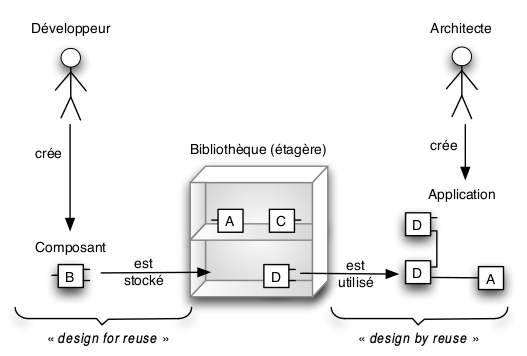
\includegraphics{images/reuse.png}
}
\caption{Vision simplifiée du processus de développement par composants, extrait de \cite{fabresse2007decoupage}}
\label{fig:reusecomponent}
\end{figure}
  
  Nous avons vu que l'architecture logicielle permettait de définir comment notre application devait être construite. C'est pour cela que nous avons besoin de visibilité sur cette architecture afin de bien appréhender comment notre application est réalisée et de visualiser toutes les intéractions entre les éléments de l'application, permettant ainsi de vérifier que cette architecture respecte bien les spécifications. Dans le développement par objets, la notion d'architecture est utilisée lors de la phase de conception de l'application. Le développeur peut se faire aider par des outils de représentation graphique, comme UML, mais cette représentation n'est que peu maintenue lors de la phase d'implémentation. Les modifications apportées par celle-ci ne sont plus visibles et donc n'assure plus que l'architecture obtenue soit conforme aux spécifications. \\\par
  
  Le développement par composants arrive à corriger cela, en rendant explicite cette visibilité sur l'architecture, soit à la manière des ADLs (Architecture Description Languages), qui permettent de décrire la structure et de définir le comportement des composants à travers leurs assemblages, par une représentation abstraite, soit directement dans l'implémentation des composants par l'approche des langages à composants, qui définissent l'architecture au sein même des composants. Par conséquent, même si pendant la phase d'implémentation on décide de modifier l'architecture de nos composants, on ne perdra pas la visibilité sur l'architecture de notre application car elle est écrite explicitement. \\\par
  
\subsection{Les grandes familles du développement à base de composants}
      
      \subsubsection{Les approches des génératives}
      
      Les approches des génératives se situent à un haut niveau d'abstraction afin de modéliser et gérer des systèmes logiciels complexes. Cette représentation se base généralement sur les ADLs, permettant de décrire les architectures à base de composants en y décrivant leurs comportements, leurs intéractions avec les autres composants et leurs configurations ainsi que leurs besoins explicites. La stratégie de cette approche générative consiste donc en la modélisation d'une architecture de composants << initiale >> décrite de manière formelle. Ensuite un << squelette >> d'application dans un langage de programmation précis qui respectera les spécifications du système est généré à partir de l'architecture. Cette représentation étant abstraite, elle est indépendante des langages de programmation qui implémentent les composants, permettant ainsi de s'adapter à tous types de plateformes. \\\par
      
      Parmi les modèles les plus importants dans cette famille, nous retrouvons UML et Fractal. \\\par
      
          \textbf{UML -- un langage de modélisation graphique pour composants}
      
      UML (Unified Modeling Language) est un langage de modélisation graphique standardisé par l'OMG (\emph{Objet management groupe}) \footnote{http://www.omg.org/spec/UML}. Dans sa première version, UML intègre déjà la notion de composant, comme étant une entité indépendante et communiquant avec d'autres composants au travers d'interfaces. La version 2.0 d'UML \cite{specificationuml} a permis d'améliorer cette vision des composants, en s'inspirant aussi des mécanismes et concepts des ADLs, introduisant la notion de port, de connecteur et de composant composite.

Un composant UML est donc une entité autonome, qui communique avec les autres composants de l'architecture au travers d'interfaces, regroupées dans des ports qui expriment des rôles. Un composant peut disposer de plusieurs ports, où un port regroupe un ensemble d'interfaces requises ou fournies. Le port permet donc de réaliser un point de communication entre l'environnement extérieur du composant et son architecture interne. 
      
 Cette connexion entre composants est permise par la notion de connecteur, qui permet de représenter les possibilités de communication entre les composants. Il existe deux types de connecteurs : d’assemblage et de délégation. Un connecteur d'assemblage permet de lier deux interfaces de deux composants. Avec une interface requise pour notre premier composant et une interface fournie pour notre deuxième composant. Cette connexion ne peut se faire que si les deux interfaces ont la même signature. Un connecteur de délégation quant à lui est utilisé afin de réaliser une connexion entre ses interfaces ou ports vers les interfaces ou ports de ses composants internes, permettant ainsi une délégation d'un besoin ou d'un service vers un composant interne.
        
    UML apporte cet aspect visuel à la représentation des architectures à composants qui manquent aux autres approches, aidant ainsi un architecte à mieux visualiser l'architecture qu'il est en train de construire. Par contre, il ne permet pas de réaliser l'implémentation et la manipulation de composants sans les coupler à une autre technique. \\\par 
    
        \textbf{Fractal -- un framework à composants intégrant un ADL}
        
        Fractal \cite{DBLP:journals/spe/BrunetonCLQS06} est une spécification d'un modèle à composants proposé par le consortium \emph{ObjectWeb} en 2002. Il propose un framework pour la création d'applications déployables sur un serveur, ainsi que la création et la manipulation de composants, intégrant en plus un ADL pour la description de l'architecture des composants. Il met en avant le concept de composant composite, de composant partagé, un mécanisme d'introspection et la possibilité de configuration dynamique. 
        
        Un composant Fractal est composé de deux parties. La partie \emph{contenu} qui est consti\-tuée des fonctionnalités que propose le composant, en étant soit un composant primitif qui dans son \emph{contenu} va implémenter la logique métier, soit un composant composite qui encapsule un assemblage de composants qui réalise les fonctionnalités attendues. La deuxième partie d'un composant est appelé la \emph{membrane}, qui contient les parties non-fonctionnelles du composant, intégrant les différentes interfaces qui communiquent avec le monde extérieur, ainsi que les interfaces qui permettent le contrôle du composant. Parmi les modèles les plus importants dans cette famille, nous retrouvons UML et Fractal. \\\par
        
        Une interface a deux types de visibilité : externe qui est visible depuis l’extérieur du composant et permettra une liaison avec d'autre composants et interne permettant une liaison avec son contenu. Une interface peut avoir différents rôles :
        
        \begin{enumerate}
        
          \item Le rôle de serveur, qui est une interface fournie proposant les différents services du composant
          
          \item Le rôle de cliente, qui est une interface requise représentant les besoins du composant
          
          \item Le rôle de contrôle, permettant la configuration dynamique du composants avec la possibilité de modifier ces liaisons avec les composants externe, de modifier son assemblage interne (modification des liaisons internes) et la gestion du cycle de vie du composant
        
        \end{enumerate}
        
        Afin de pouvoir connecter des composants entre eux, il faut connecter une interface de l'un avec une interface de l'autre. Cette connexion est appelée liaison (\emph{binding}) et peut être de trois types : une liaison normale (\emph{normal binding}) entre une interface serveur externe d'un composant et une interface cliente externe d'un autre composant, une liaison d'export (\emph{export binding}) entre une interface cliente d'un composite et une interface serveur d'un composant interne, permettant donc la délégation d'un service fourni par notre composant composite qui sera fourni par son composant interne, et une liaison d'import (\emph{import binding}) entre une interface serveur interne d'un composant composite et une interface cliente externe d'un composant interne permettant la délégation d'un besoin de notre composant interne au composant composite.
        
        Étant un modèle abstrait, il permet de s'abstraire de tous langages et de plateformes pour la gestion de composants. Différentes implémentations ont été réalisées (par exemple en Java avec Julia ou en C++ avec Cecilia). En effet l'ADL qu’intègre Fractal est décrit dans une syntaxe XML et spécifié de manière indépendante des langages de programmation. Les différentes implémentations proposent cependant un mécanisme de génération de code à partir de l'ADL pour réaliser l'implémentation des composants. \\\par

    \subsubsection{La famille des frameworks}     
   
    La famille des frameworks à composants utilise les langages de programmation à objets connus, pour la création et la manipulation de composants afin de modéliser un système. Cette approche permet au développeur d'utiliser les composants afin de bien séparer les besoins fonctionnels et les besoins non-fonctionnels. Principalement utilisé dans le monde professionnel, les frameworks à composants proposent aux développeurs de créer, déployer et configurer une application.  \\\par
    
    Parmi les frameworks les plus importants dans cette famille, nous retrouvons Enterprise JavaBeans et Spring. \\\par
    
    \textbf{Enterprise JavaBeans -- un framework à composants pour la création d'applications distribuées} 
    
    L'approche de composant mise en place par Enterprise JavaBeans (EJB), développée au sein de la plateforme Java Enterprise Edition (JEE), propose un modèle à composants serveur permettant la réalisation d'applications distribuées \cite{specificationejb}.
    
    Un composant EJB s’exécute dans un conteneur au sein d'un serveur JEE. Les conteneurs gèrent les instances des EJB, tandis que le serveur fournit au conteneur des besoins non-fonctionnels.
    
    Un composants EJB est regroupé en trois catégories : session, entité et message. Une instance d'un composant entité permet de représenter un concept métier, ayant pour but de représenter des données pouvant être stockées dans une base de données. Une instance d'un composant message permet la gestion de messages asynchrones reçus par le serveur depuis le client. Une instance d'un composant session permet de fournir des services définis par des méthodes, pouvant être sans état (stateless) ou avec état (stateful).
    
    Un composant EJB communique ses services par une interface \emph{remote}, spécifiant ainsi les méthodes que fournit une instance d'un EJB au monde extérieur. Il permet sa configuration et la gestion de son cycle de vie par une interface \emph{home} qui est fournie par son conteneur. Cependant on ne peut définir le besoin d'un EJB au moyen d'une interface requise. Les propriétés d'un EJB sont définies dans un descripteur de déploiement permettant au conteneur EJB de savoir comment gérer les composants pendant leur exécution.
    
    L’approche des EJB ne permet pas la réalisation de composant composite. Ainsi une architecture sera dite << à plat >>, chaque composant sera au même niveau que les autres, permettant une vision horizontale de l'architecture. Mais cela peut s’avérer répétitif de réaliser l'ensemble de toutes les différentes connexions entre composants sans pouvoir utiliser la composition pour réutiliser un assemblage de composants. \\\par
    
    \textbf{Spring -- un framework à composants pour la création d'applications modulaires}
    
    Spring \footnote{https://spring.io/} est un framework utilisé afin de fournir une infrastructure compréhensive pour la création d'applications Java. Comme la grande majorité des frameworks, il fonctionne sur le principe de l'inversion de contrôle (IoC -- patron de conception où le processus d’exécution d'une application est géré par le framework), qui est assurée par la recherche de dépendances et l'injection de dépendances automatique, tout en offrant un ensemble de fonctionnalités facilitant l'accès aux données, le développement web, les tests automatisés, etc., qui sont organisés en modules.  
    
    Un module est une unité de code indépendante d'un système logiciel. Il possède deux caractéristiques fondamentales~:  une forte cohésion (le module se focalise sur une tâche unique), et un couplage minimal (le module a de faibles dépendances avec les autres modules). Un module est décrit par une spécification, qui définit les signatures des fonctions publiques fournies par le module et une implémentation, qui implémente les fonctions fournies. Il permet de répondre aux problématiques de maintenabilité, réutilisabilité et testabilité. 
    
    Le cœur de Spring est géré par le \emph{Spring Core Container}, qui est un ensemble de modules permettant la réalisation du conteneur Spring de l'application, qui a un comportement similaire au conteneur EJB. Il implémente l'IoC et permet de gérer la création, le cycle de vie et les dépendances des \emph{bean} qu'il contient (un composant Spring (bean) étant une classe Java qui implémente une ou plusieurs interfaces fournies). La description des beans est principalement décrite dans des fichiers XML mais peut se faire dans le code source avec l'utilisation d'annotations Java ou l'utilisation de code source de manière spécifique par le framework.
    
    Cette description décrit la classe du bean, ainsi que son identifiant. On peut injecter à cette description des constructeurs, avec comme argument des valeurs primitives ou des références vers d'autre beans (grâce à par leur identifiant). On peut aussi rajouter un ensemble de propriétés (i.e. attribut privé ayant un getter et un setter), définis par un nom et une valeur d'un type primitif ou une référence vers un autre bean. La reconfiguration d'un bean (par exemple, modifier la référence vers un bean d'une propriété), se réalise par la modification textuelle de la référence et la relance de l'exécution de l'application. Un bean composite est obtenu par la déclaration d'un bean interne (inner bean), qui se comporte comme une classe interne. \\\par 
             
    \subsubsection{La famille des langages à composants}
    
    \label{sec:presentcomponent}
    
    L'approche des langages à composants s'articule autour d'un seul langage de programmation pour permettre de définir une architecture de composants et l'implémen\-ta\-tion de ses composants. Ce regroupement de ses deux principes permet de faciliter le développement, car le programmeur ne doit connaître qu'un seul langage.  
    Cette approche autour d'un seul langage permet de ne pas avoir de violation de contraintes architecturales, qui pouvait se produire avec les ADLs, qui ont une description dans un langage et l'implémentation dans un autre.\\\par 
    
    Parmi les langages à composants les plus importants dans cette famille, nous retrouvons ArchJava et ComponentJ. \\\par
    
      \textbf{ArchJava -- un langage à composants} 
      
      ArchJava \footnote{http://www.archjava.org/} créé en 2001 \cite{DBLP:conf/icse/AldrichCN02}, s'inspire de l'approche composant que proposent les ADLs pour la description d'architecture, tout en permettant l'implémentation de ces composants au sein d'un nouveau langage qui est une extension du langage Java.
      
      Un composant est dans ce monde un <<objet particulier>>, qui s'obtient par instanciation de la classe \texttt{component class}. Cette classe de composant permet de regrouper les informations du composant : ses ports, ses méthodes, ses attributs, ainsi que ma description de son assemblage interne à travers des connexions.
      
  Deux composants ne peuvent communiquer entre eux que s'ils sont explicitement connectés par la primitive \texttt{connect}. Cette primitive introduit la connexion entre composants par la liaison de leurs ports respectifs pour la première fois dans l'histoire des approches à composants 
  
 Un port définit une liste de méthodes fournies et requises, différenciées respectivement par les primitives \texttt{provides} et \texttt{requires}. Une méthode fournie permet d'introduire une fonctionnalité proposée par le composant au monde extérieur. Les autres composants n'ont accès à cette méthode que par le biais du port. Une méthode requise permet de décrire une fonctionnalité attendue par notre composant. Deux ports ne peuvent se lier entre eux que si les signatures des méthodes requises et fournies qu'ils définissent sont compatibles entre eux. \\\par 
  
  \textbf{ComponentJ -- un langage à composants} 

  ComponentJ \footnote{https://projectos.fct.unl.pt/projects/di-componentj/wiki} présenté par \cite{seco2008component}, propose un modèle à composants, explicitant les dépendances entre composants, la création dynamique de nouveaux composants, la reconfiguration au runtime et un typage fort pour les composants. Il ne faut pas le confondre avec son cousin ArchJava, qui comme lui est une extension du langage Java, car ils sont tous les deux conceptuellement différents.

  Par exemple, un composant est un élément instance d'une classe dans ArchJava, alors qu'un composant est un descripteur instanciable d'objets en ComponentJ. Ce descripteur permet de définir la structure et le comportement de chacune de leurs instances en décrivant les ports et en définissant les services fournis par les objets. En effet, un objet en ComponentJ est une instance de composant, qui a un comportement comparable à un objet Java. Cependant il doit être typé par une interface (\textbf{object interface}) qui définit l'ensemble des services que fournira notre objet, à travers la définition d'un seul port fourni.
    
  Les ports sont des interfaces (\textbf{port interface}) qui définissent un ensembles de signatures de méthodes. Ces méthodes représentent les services des composants et seront dites requises ou fournies en fonction du rôle du port qui les définit. En effet si un port a un rôle de fourni dans un composant alors ce composant devra implémenter ces méthodes, identifiées par la primitive \texttt{methods}. Tandis que si un port a un rôle de requis, alors le composants pourra invoquer ces méthodes afin de les utiliser. 
  
  Les configurateurs sont des blocs d'instructions présents dans les composants. Ils permettent le mécanisme de composition ou de connexion. Ils peuvent être utilisés pour la création au runtime de nouveaux composants, ainsi que la reconfiguration des comportements et la restructuration des composants.
  
  ComponentJ a fait le choix de mettre en avant l'assemblage de composants, qui ne sont pas ici des instances mais des descripteurs, leur instanciation étant possible uniquement si les dépendances requises sont satisfaites ce qui permet d'avoir une forte sûreté à l'exécution, mais rend plus contraignante l'utilisation des composants. En effet, un développeur doit satisfaire l'ensemble des besoins de chaque composant, même ceux qui seraient inutiles dans l'application. \\\par
  
  

    
      


  \section{Les différents mécanismes du passage d'arguments en programmation}

        \subsection{Terminologie}
    
      \label{sec:arguments}
            
   Dans la majorité des langages de programmation, l'appel à un sous-programme (procé\-dure, fonction, méthodes, etc.) peut prendre des paramètres en arguments. On ne s'inté\-resse ici pas en détail sur le fonctionnement de cet appel, mais on se concentrera sur comment un paramètre effectif est transmis au sous-programme et comment son utilisation dans le corps du sous-programme peut dans certains cas impacter l'environnement. Il existe un grand nombre de mécanismes de passage d'argument mais nous allons essayer de voir les plus connus et les plus utilisés, présentés dans \cite{Horowitz:1984:FPL:27635}.
  
    \subsection{Passage par valeur}
      
      Sûrement le mécanisme de passage d'arguments le plus connu et utilisé, le passage d'argument est appelé << par valeur >> quand des modifications sont apportées aux paramètres formels et n'ont aucun impact sur l'environnement extérieur et ne modifient en aucun cas l'état du paramètre effectif. Dans ce mode de passage, le paramètre effectif est déréférencé donnant une \emph{r-value} \footnote{contenant une variable ou le résultat d'une expression} qui est copiée dans une nouvelle zone mémoire, liée à notre paramètre formel. Cependant cette copie consomme de l'espace mémoire et du temps de calcul pour la copie. Un grand nombre de langage utilise ce mécanisme, comme un mécanisme par défaut, notamment C, C++ \cite{Stroustrup:2000:CPL:518791}, ou encore Java.

    \subsection{Passage par référence}
    
     Dans le mécanisme de passage par référence, le paramètre formel fait référence à l'adresse mémoire de notre paramètre effectif. Dans ce mécanisme aucune copie n'est réalisée, ce qui permet de ne pas avoir les contraintes du passage par valeur, car aucune nouvelle zone mémoire n'a besoin d'être allouée. Toutes les modifications auront un impact sur l'environnement local à la fonction mais aussi sur l'environnement extérieur à celle-ci.  
    
    Java \cite{Gosling:2005:JLS:1036643} utilise le passage par valeur pour les objets. En effet, même si certain affirmeront que Java fait un passage par référence, c'est en fait un abus de langage, c'est-à-dire que techniquement c'est un passage par valeur qui entraîne une copie de la référence de notre paramètre effectif. On se retrouve alors avec deux références qui pointent vers la zone mémoire de notre objet, ce qui a pour conséquence que si on réalise un envoie de message qui modifie un attribut d'un objet passé en paramètre cela entraînera une modification sur le paramètre effectif. Mais si on réalise une affection sur cet objet alors le paramètre formel référencera une nouvelle zone mémoire, et les nouvelles modifications de l'état de notre objet ne modifieront plus l'état de notre paramètre effectif, car feront référence à la nouvelle zone mémoire créée. 
      
    \subsection{Passage par valeur-résultat}
    
    E. Horowitz définit le passage par << value-result >> \cite{Horowitz:1984:FPL:27635} comme une méthode incluant les fonctionnalités du passage par valeur et du passage par référence. Dans ce type de passage, dans le corps du sous-programme le paramètre formel a le même mécanisme que le passage par valeur, avec déréférencement du paramètre effectif et la copie dans une nouvelle zone mémoire. Durant toute l'exécution du sous-programme les modifications n'auront un impact que sur l'environnement local de la fonction, mais une fois celle-ci terminé, la valeur du paramètre formel est copiée vers celle du paramètre effectif. Ce mécanisme est utilisé par le langage ALGOL-W \cite{sites1972algol} (une variante d'Algol60).
    
    \subsection{Passage par nom}
    
  Dans ce mécanisme de passage de paramètres, c'est une substitution textuelle qui est effectuée dans le corps de la fonction à chaque fois que le paramètre formel apparaît par le paramètre d'effectif. Ce comportement est introduit comme comportement par défaut en ALGOL-60. Il réalise un effet semblable au passage par référence, dans le sens où aucune copie n'est réalisée et son champ d'action impacte aussi l’environnement extérieur. Il est aussi comparable aussi au macro en C.
    
    \subsection{ADA et ses trois nouveaux mode de passage}
   
   Le passage de paramètres en ADA est un peu particulier. En effet, comme mentionné par J-L. Nebut \cite{opac-b1077467}, le programmeur ne peut pas choisir entre un passage par valeur ou référence (les deux mécanismes présents dans ADA), mais a la possibilité de choisir un << mode >> de passage. Le mode permet au développeur de définir chaque argument comme étant en entrée (IN), sortie (OUT) ou entrée/sortie (IN OUT).

En mode \texttt{IN}, le paramètre formel est vraiment en << read-only >>, c'est-à-dire que dans le corps de la fonction on ne peut pas modifier la valeur du paramètre formel. C'est le comportement par défaut utilisé par ADA. En mode \texttt{OUT}, le paramètre formel peut être modifié dans la procédure mais ne peut être lu. Si le paramètre effectif est affecté dans la procédure, sa valeur pourra être utilisée dans la suite du programme avec cette nouvelle valeur affectée. En mode \texttt{IN OUT}, les deux mécanismes précédents sont combinés, avec comme contrainte que le paramètre effectif doit être initialisé avant l'appel.
    
    

  
  \section{La sémantique formelle des langages de programmation}
  
    
  \subsection{Présentation}
  
    La sémantique d'un langage de programmation permet de définir le comportement d'un programme écrit dans ce langage, à la différence de la syntaxe d'un langage de programmation qui permet de décrire la représentation d'un programme dans ce langage. Ces deux notions sont complémentaires mais la frontière entre la sémantique et la syntaxe n'a pas toujours été claire (notamment dans les années 70). Cependant les travaux de C. Strachey et D. Scott ont été fondateurs pour la séparation de ces deux domaines. On peut citer notamment C. Strachey qui disait :
  
  \begin{quote}
      \emph{La sémantique est là pour ce que nous voulons dire et la syntaxe
pour comment nous avons à le dire. } C. Strachey
  \end{quote}
      
  De manière générale, les concepteurs de langage de programmation définissent la sémantique de leur langage de manière informelle, au moyen de blocs de texte, écrits en langage naturel, ce qui laisse la place à l'ambiguïté, lors de l'interprétation d'un comportement décrit dans cette sémantique informelle. Pour éviter toute ambiguïté, les sémantiques formelles reposent sur l'utilisation des mathématiques afin d'exprimer rigoureusement le comportement des programmes.\\\par
        
        Les motivations derrière la formalisation de la sémantique d'un langage sont nombreuses. Cela permet de visualiser tout comportement possible à l'exécution (même les cas d'erreurs), de lever toute ambiguïté pour un utilisateur du langage (car décrit formellement), de démontrer différentes sémantiques pour un même langage, l'équivalence de programmes (syntaxiquement différents), la validation de transformations de programme, des propriétés relatives au typage (comme la correction du typage par rapport à la sémantique ou la préservation du typage lors de l'exécution). Cela permet aussi le développement d'outils certifiés (interprètes, compilateurs, analyseurs statiques, etc.).
      
      \subsection {Les grandes approches de la sémantique formelle}
      
      Dans la littérature on remarque trois grandes approches de la sémantique formelle \cite{Winskel:1993:FSP:151145}~, décrites aussi par Xavier Leroy \footnote{http://cristal.inria.fr/$\sim$xleroy/mpri/prog/cours.pdf}.
      
      \begin{enumerate}
      
        \item La sémantique axiomatique, reposant sur la logique de Floyd-Hoare, permet de décrire le comportement des programmes impératifs annotés par des assertions (formule logique). Elle permet d'assurer la validité des valeurs des variables avant et après l'exécution, si les instructions terminent. 
        
        \item La sémantique dénotationnelle est la première sémantique à avoir été introduit (début 70) par C. Strachey et D. Scott. Elle met en relation une instruction du programme avec sa dénotation. La dénotation est généralement une fonction, au sens mathématique du terme, c'est-à-dire associe des entrées à des sorties (plus généralement un domaine à un autre -- théorie des domaines). Permettant de décrire de façon précise la sémantique du langage mais de façon la plus abstraite possible, elle reste toutefois difficile à manipuler et à implanter. 
        
        \item La sémantique opérationnelle met en relation un programme avec son résultat. Cette relation peut être de deux natures : <<à grands pas>> (dite <<à la Kahn>>) ou <<à petits pas>> (dite <<à la Plotkin>>). Cette sémantique opérationnelle est donnée par un ensemble de règles d'inférence, reposant sur des structures inductives (théorie des types). 
        La sémantique à grands pas met directement en relation un programme avec son résultat, ne montrant pas les étapes intermédiaires de calculs. Elle est sans doute la sémantique la plus proche d'une implantation. En revanche, elle parle plus difficilement des programmes qui ne terminent pas. Cet type de programmes peut être caractérisé plus facilement avec une sémantique à petits pas, qui décrit toutes les étapes intermédiaires de calcul entre le programme et le résultat final. Toutefois, les sémantiques à petits pas restent plus loin d'une implantation et sont moins efficaces en pratique.
      
      \end{enumerate} 
         
    \subsection{Mécanisation des sémantiques formelles}
      
        Pour nous aider dans la formalisation des sémantiques, différents outils d'aide à la preuve existent. Par exemple, Coq \footnote{https://coq.inria.fr/} est un outil développé au sein de l’équipe INRIA $\pi$$r^{2}$ et fondé sur la théorie des types (calcul des constructions inductives). Coq est particulièrement approprié pour formaliser les sémantiques car il propose un très bon support pour les types inductifs. En effet, les types inductifs sont un moyen idiomatique de formaliser en Coq, et permettent en particulier de traduire presque directement les sémantiques opérationnelles exprimées sous la forme de règles d'inférence. Par ailleurs, il existe également des outils en Coq \cite{Rel-Exec3} permettant d'extraire des interprètes à partir de la formalisation de sémantiques exprimées au moyen de types inductifs, ainsi que les preuves de correction correspondantes (c'est-à-dire que les interprètes extraits sont conformes aux sémantiques formalisées). Il existe également d'autres outils d'aide à la preuve qui possèdent un bon support pour l'induction et qui sont aussi appropriés pour la formalisation de sémantiques. On pourra citer en particulier Lego~\footnote{http://www.dcs.ed.ac.uk/home/lego/} ou Isabell~\footnote{https://isabelle.in.tum.de/}.
        
  \subsection{La sémantique formelle des langages objets et des langages à composants}
  
       Il existe assez peu de travaux sur la formalisation de la sémantique des langages à objets et la référence en la matière sont les travaux de M.~Abadi et L.~Cardelli \cite{Abadi:1996:TO:547964}, qui ont proposé une nouvelle approche dans la compréhension des langages objets, en présentant des calculs d'objets et développant une théorie  autour d'eux, en couvrant leurs sémantiques et leurs règles de typages.
      
      Cependant il n'existe pas, à notre connaissance, de travaux autour de la formalisation de la sémantique des langages à composants, sauf quelques rares exceptions comme~\cite{peschanski2001typeful}.
        
      

        
\chapter{Problématique du stage de recherche} 

  \section{Le langage orienté composant, Compo} 
  
        
    \label{sec:compo} 

    Développé au sein de l'équipe MAREL du LIRMM, le projet Compo\footnote{http://www.lirmm.fr/compo/} est un travail de collaboration et de réflexion autour du développement d'un langage pur composants, promu par son créateur C.Dony avec l'aide de C.Tibermacine et D.Delahaye, ainsi que des travaux de recherche réalisés dans les thèses de P.Spacek \cite{Spacek:2014:CMA:2602458.2602476} et L.Fabresse \cite{fabresse2007decoupage}.
    
    \subsection{Compo -- un langage tout composant}
    
L'idée du langage Compo est d'unifier les concepts des précédentes approches à composants autour d'un langage de programmation. Il s'inspire des ADLs, pour une description explicite des architectures, ainsi que l'idée de pouvoir définir explicitement le requis d'un composant. Il reprend le concept des LOC de mettre au même niveau une description de l'architecture et l'implémentation des composants. De la même manière que l'approche de UML, il permet une visualisation graphique de l'architecture interne d'un composant. Avec la même philosophie que Smalltalk pour un monde <<tout objet>>, Compo prône un monde <<tout composant>>. Dans sa deuxième version de développement, Compo a intégré la réflexivité au sein de son méta-modèle, réalisée par les travaux de P.Spacek \cite{Spacek:2014:CMA:2602458.2602476}, décrivant les descripteurs, ports et services comme étant des composants. 
  
      \subsubsection{Composants et descripteurs}
    
    Un composants Compo est décrit par son descripteur, dont il est instance. Un descripteur permet de définir la structure et le comportement de chacune de ses instances en décrivant les ports et l'architecture et en définissant les services. 
    
      \subsubsection{Des ports comme seul moyen de communication entre composants}
      
     Un port regroupe un ensemble d'interfaces (fournies ou requises). Comme l'approche de Fractal ou ComponentJ, les ports de Compo sont unidirectionnel, c'est-à-dire qu'un port est soit un ensemble d'interfaces fournies, on parle alors de port fourni (\texttt{provides}), soit un ensemble d'interfaces requises, on parle alors de port requis (\texttt{requires}). Contrairement aux ports bidirectionnels, les ports permettent un découplage du requis et du besoin entre composants. En effet les approches comme Archjava ou en UML, les ports sont un ensemble d'interfaces fournies et/ou requises, laissant plus de souplesse dans le développement mais introduisant une perte de sécurité au niveau l'architecture. En effet, un composant fournissant un service n'a pas forcement besoin d'avoir accès au service du composant auquel il se connecte. Il possède aussi une visibilité, interne ou externe. Par défaut un port est externe, visible depuis l'environnement extérieur. Un port peut devenir interne, visible uniquement dans l'environnement interne du composant, grâce à l'ajout de la primitive \texttt{internally}.
    
    \subsubsection{Les services}
    
    Un service est représenté par un nom et un ensemble de paramètres. Il représente une fonctionnalité que peut fournir chaque composant qui est instance du descripteur qui le définit. L'invocation du service d'un composant se réalise au travers d'un port requis du composant. Il peut aussi être défini dans des descripteurs de composants composites. Ainsi un composant composite encapsule un assemblage de composants et peut y rajouter des comportements grâce à des services. Ceci n'est pas possible dans les approches comme Fractal par exemple, où la définition de service ne peut se faire que par des composants primitif.
    
    \subsubsection{Une description d'architecture explicite}
      
      Cette description d'architecture est contenue dans un bloc d'instructions, identifié par la primitive \texttt{architecture}. Elle permet de représenter les connexions entre les composants internes de notre composant avec l’instruction \texttt{connect} et de permettre la délégation, entre un port externe fourni (resp. requis) de notre composant à un port externe fourni (resp. requis) d'un composant interne, avec l'instruction \texttt{delegate}.
      
    \subsubsection{Des composants composites}
      
    Compo intègre lui aussi la notion de composant composite, comme le font certaines des autres approches. Cependant, contrairement à ArchJava qui encapsule les composants internes de la même façon qu'une classe peut le faire avec ses attributs, Compo stocke ses composants internes à l'aide de ports internes requis. Une instance d'un composant interne est liée à ce port requis interne par son port fournis externe.
  
    \subsection{Compo -- une architecture à composants d'un compteur}
    
    L'annexe \ref{ann:compoexemple} permet de décrire une architecture de composant qui simule le comportement d'un compteur. Le premier composant est décrit par le descripteur \texttt{Printer}. Il décrit le service \texttt{print}, qui permet d'afficher une chaîne de caractères. Le deuxième composant est décrit par le descripteur \texttt{Counter} qui permet de simuler l'incrémentation d'un compteur au travers de son service \texttt{increment}. Cette même valeur est encapsulée dans notre composant par un composant \texttt{Integer}. Notre composant a aussi besoin d'être connecté à un autre composant lui fournissant le service \texttt{print}.Le dernier composant est décrit par le descripteur \texttt{PrintableCounter} qui décrit notre architecture de composants. Il encapsule nos deux composants et leurs connexions (ligne 62). Le service $main$ qu'il fourni, aura comme comportement d'incrémenter le compteur et d'afficher sa valeur.  
    
      
      
      


      
      

    
  \section{La problèmatique du passage des arguments dans les modèles à composants}
    
      
  \label{sec:argumentscomposants}
  
  \subsection{La signification du passage d'un composant en argument}
  
  Les composants peuvent avoir besoin de s'échanger des données. Dans les autres approches et notamment les autres LOC ces données sont des objets, il est donc normal de se demander comment un composant passe à un autre composant une donnée, sachant que cette donnée est aussi un composant. Le composant A qui voudrait passer en argument un composant C à un service du composant B qu'il invoque, permettrait une connexion entre le composant C et le composant B (représenté dans figure \ref{fig:archiCompo}). Le mécanisme de cette connexion étant décrit par \cite{Spacek:2014:CMA:2602458.2602476} : 
  
  \begin{quote}
      \emph{\textbf{Choice 17 : }Arguments passing is made by the automatic establishment and removal of connections. Any component has a required collection port named args . During a service invocation, the arguments, i.e. ports, {a1, a2, ..., an} are each respectively connected to {args[1], args[2], ..., args[n]}. The identifiers of the parameters are actually alias identifiers of ports args . At the end of the execution of the service, all connections to args ports are removed. In the case when a service invocation is delegated, because the receiving port is delegated, the appropriate delegation connection for the args port is also automatically established and removed} 
  \end{quote}
  
\begin{figure}[!t]
\centering
\scalebox{.5}{
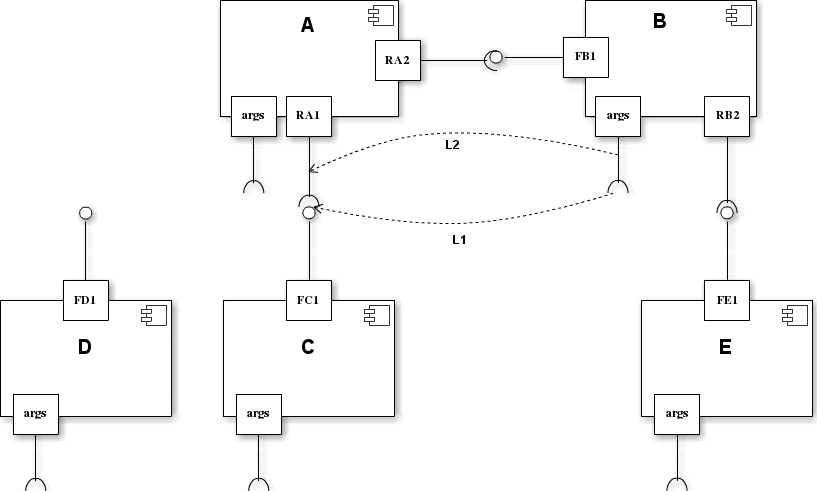
\includegraphics{images/archiCompo.png}
}
\caption{Exemple du passage en arguments d'un composant}
\label{fig:archiCompo}
\end{figure}
  
  \subsection{Les premières pistes du passage d'arguments}
  
      \subsubsection{Le passage par fourni}
      
      Une connexion par port fourni (ou passage par fourni), figure \ref{fig:archiCompo}, est représenté par la liaison \emph{L1} entre le port \emph{args[1]} du composant B et le port fourni \emph{FC1} du composant C. Cette connexion entre B et C permet au composant B d'avoir accès au service de C, cependant on remarque que le composant A n'a plus de contrôle sur cette connexion car elle ne passe plus par lui. De plus si jamais le composant A décide de modifier sa connexion à C vers un autre composant (ici D par exemple), alors B gardera la connexion vers C, créant ainsi un comportement parallèle. Ce comportement peut s'avérer utile dans certain cas, par exemple si A modifie sa connexion plusieurs fois, il permettrait à B de conserver des connexions vers les anciens arguments de A (permettant ainsi d'avoir un historique des connexions). 
      
      \subsubsection{Le passage par requis}
      
      Une connexion par port requis (ou passage par requis), figure \ref{fig:archiCompo}, est représenté par la liaison \emph{L2} entre le port \emph{args[1]} du composant B et le port requis \emph{RA1} du composant A. Cette liaison met en place un mécanisme de délégation entre le port de A et le port de B. Cela permet à B d'invoquer les services de C, tout en permettant à A d'avoir un possible contrôle sur cette connexion, car elle passe par son port. De plus si jamais A modifie sa connexion à C vers un nouveau composant, alors B aura lui aussi cette connexion vers D. Cela permet donc la création d'architectures très réactives aux changements de composants, ce qui fait défaut au passage par fourni. 
      
  \subsection{Comparaison avec les passages d'arguments classiques}
  
  Nous avons vu précédemment les différents mécanismes de passage d'argument qui pouvaient exister dans les langages de programmation. Il est intéressant de se demander comment ces différents mécanismes pourraient se traduire dans un passage de composant en arguments. 
   
  On peut faire un premier parallèle du passage par fourni, qui semble permettre un mécanisme similaire au passage de référence en Java. En effet les modifications de l'état du composant C dans le service de B auront un impact sur le composant C. De plus si A modifie sa connexion vers C vers un autre composant et que B a conservé sa connexion vers C alors comme en Java B n'aura pas une référence vers D mais toujours vers C.
  
  Le passage par requis ne peut pas se réaliser en Java, mais on peut avoir un comportement qui s'en rapproche en C++ par un référencement vers un pointeur. Si un objet A passe par référence un pointeur $c$ à une méthode $foo$ de B, et que B conserve cette référence dans un pointeur $var$, alors $var$ aura comme référence l'adresse du pointeur $c$. Ainsi si A modifie la référence du pointeur $c$, alors B aura bien une référence vers un pointeur qui fera référence à ce nouvel objet.
  
  \subsection{Les potentialités découlant du passage par requis comme support au passage d'arguments}

    Le passage par requis permet déjà des potentialités sur cette connexion pour le passage en arguments, et qui demanderait peu de modifications afin d'être implémenté. 
  
      \subsubsection{Un passage en lecture seule}
    
   Une connexion en mode <<read-only>> permettrait en effet de pouvoir passer un composant C à un composant B, où B ne pourrait pas modifier l'état du composant C, c'est-à-dire invoquer seulement des services de C qui n'ont pas un impact sur l'état de C, comparable à l'utilisation du mot clé const de C++. On peut donc imaginer la mise en place d'une nouvelle propriété sur les ports qui indiquerait s'ils sont en mode <<read-only>> ou non et de pouvoir modifier cette propriété selon le besoin. On peut aussi imaginer un nouveau type de port qui ne permettrait que le passage en <<read-only>> et le composant A devrait choisir quel type de port il veut utiliser. Ce mécanisme <<read-only>> peut cependant être réalisé manuellement par la mise en place d'un composant placé entre nos deux composants, qui filtrerait les services que peut invoquer notre composant.
  
      \subsubsection{Un passage révocable}
    
    Nous avons vu que le passage par requis permettait au composant A d'exercer un contrôle sur la connexion de B vers C. On peut donc imaginer là aussi une nouvelle propriété ou un nouveau type de port permettant de <<couper>> la connexion entre B et C mais aussi de pouvoir la rétablir selon le besoin. La difficulté de la propagation d'un passage révocable par le passage par requis est minime, si B passe C en argument au composant E, alors supprimer la délégation entre le port de A et le port B, supprimera la délégation implicite de E vers C. \\\par
    
  \subsection{De nouvelles pistes ouvertes par les résultats de recherches récentes}
  
    \subsubsection{Les références comme entité de première classe}
    
    Faire des références une entité de première classe permet d'exercer un contrôle sur les références des objets, permettant de construire des systèmes objet avec une plus grande sécurité. En apportant des comportements comme des références en lecture seule, révocables. On pourra notamment regarder les travaux portant sur les langages à typage statique \cite{DBLP:conf/oopsla/ClarkePN98} ou encore les travaux de \cite{DBLP:journals/scp/ArnaudDDT15} portant sur les langages à typage dynamique. 
    
    Cependant on pourra discuter de la propagation du contrôle des références, en regardant un exemple inspiré de \cite{DBLP:journals/scp/ArnaudDDT15}. Un objet A passe une référence révocable vers un objet C à un objet B. Cependant B a aussi une autre référence indirecte vers C en passant par D. Alors si A révoque la référence révocable vers C, cela a-t-il un impact sur la référence indirecte vers B ?
    
    On pourra aussi regrouper les travaux de \cite{DBLP:conf/oopsla/Abi-AntounA06}, qui essaye de lutter contre l'aliasing, en contrôlant les échanges de références, en regroupant les objets dans des domaines et en explicitant les lien entre eux. Mettant aussi en place des mots clés permettant de gérer les droits d'accès des objets, comme \textbf{unique} (ne peut être pointé que par une seule référence), \textbf{owned} (ne peut être accessible que par des objets du même domaine), \textbf{shared} (partagé entre les domaines).
    
    On remarque cependant que ces différents mécanismes se retrouvent conceptuellement dans les ports de Compo, et pourraient être implémentés sans demander un grand effort de conception, par l'ajout de nouveaux types de ports par exemple.
    
    \subsubsection{La réification des connecteurs}
 
    Un connecteur permet de représenter la sémantique d'une connexion entre deux ou plusieurs instances. Cependant les langages à objets ne permettent pas de fournir une représentation explicite des connexions entre instances, car étant implicitement comprises dans leurs références. Dans le monde composant cette connexion est explicitement décrite et représente une liaison entre deux ou plusieurs éléments connectables (e.g. ports ou interfaces) \cite{IversDocumentingComponent2004}.
    
    \cite{DBLP:conf/ecoop/AldrichSCN03} propose donc d'intégrer les connecteurs au LOC ArchJava, afin de permettre au développeur de pouvoir modifier la sémantique d'un connecteur à l’exécution et de modifier le comportement de vérification de type entre les ports. 
    Par défaut la compatibilité de deux interfaces est la même que dans Java, cependant ajouter un nouveau connecteur qui hérite de la classe $Connector$ et surcharger sa méthode $typecheck$, permet de modifier la vérification de cette compatibilité. 
    Par exemple, dans \cite{DBLP:conf/ecoop/AldrichSCN03}, un nouveau connecteur $TCPConnector$ est défini, ne supportant une conne\-xion qu'entre exactement deux ports et l'ensemble des arguments doivent être des sous-types de l'interface $Serializable$ de Java. Le développeur peut ensuite s'il le désire lors de la définition d'une connexion (\textbf{connect}), spécifier un connecteur particulier (\textbf{with new} [{\itshape connecteur}])
    
    Réifier les connecteurs dans Compo ne serait que redondant car leur mécanisme est déjà incorporé dans les ports. Cependant la possibilité de pouvoir ajouter un nouveau comportement de vérification peut être utile dans certains cas d'utilisation et se réaliserait par l'utilisation d'un nouveau type de port. 

  \subsection{La signification du retour d'un composant à une invocation de service}
  
      En complément des interrogations sur le passage de composants en arguments, il est intéressant de se demander ce que signifie retourner un composant suite à une invocation de service. Une connexion est aussi réalisée entre le composant retourné et le composant qui réalise l'invocation. On prendra comme exemple, le composant E qui serait le retour d'un invocation de service du composant B par le composant A, figure \ref{fig:archiCompo}.
  
      Dans le cas d'un retour par port fourni (ou retour par fourni), le même mécanisme de connexion est utilisé entre les ports de nos composants. Alors, une connexion entre un port requis de A et le port fournis $FE1$ de E est mise en place, donnant ainsi une connexion directe vers le composant E au composant A sans avoir à passer par B. 
  
      Dans le cas d'un retour par port requis (ou retour par requis), le même mécanisme de délégation est utilisé entre les deux ports requis. Ainsi, une délégation entre un port requis de A et le port requis $RB2$ est mise en place, donnant ainsi à B le contrôle sur la connexion entre A et E.
         

    
  \section{Formaliser la sémantique de Compo}
    
      \subsection{Évolution du noyau sémantique existant et formalisation des nouveaux mécanismes}
  
  La première étape de la formalisation de la sémantique du langage Compo, consiste en la définition des règles d'inférence. Partant d'une base de règles déjà définie par D.Delahaye, nous devrons continuer la définition des règles d'inférence pour prendre en compte l'ensemble des mécanismes de Compo, qui ce réaliserons sur papier au cours de cette première étape. Cette définition portera cependant sur un noyau de Compo non réflexif, qui sera intégré dans de futurs travaux. \\\par
  
  Nous avons vu précédemment que la réflexion autour de la problématique du passage en argument d'un composant nous suggère différentes pistes. Ainsi la formalisation des différents modes de passage nous apportera un regard neuf dans le choix du mode et de pouvoir comparer les modes entre eux en définissant formellement leur comportement.
    
  \subsection{Mécanisation en Coq et génération d’un interprète certifié}
  
  La deuxième étape se réalisera avec l'outil Coq, qui mécanisera les règles d'inférence au moyen de type inductif. Le choix de Coq comme outil pour la mécanisation se justifie par le fait qu'il est particulièrement efficace pour formaliser une sémantique opérationnelle exprimé sous la forme de règles d'inférence. De plus au cours de ma formation j'ai eu location de l'utiliser afin de mécaniser la sémantique d'un mini-langage fonctionnel.
  
  Le but ultime à atteindre serait l'extraction d'un interprète certifié, qui peut se réaliser à l'aide d'un plugin développé par D.Delahaye et un doctorant \cite{Rel-Exec3}.
  .

    
\chapter{Conclusion} 

    Rappelle du sujet avec les objectifs et les buts à atteindre

  Approche originale de la sémantique formelle d'un langage à composant 
  
  Avenir de Compo.

  
\appendix 
  \clearpage
	\phantomsection
	
  \chapter{Une architecture composant d'un compteur en Compo}
    
    \label{ann:compoexemple}
  
    \lstinputlisting[numbers=left,breaklines=true,basicstyle=\footnotesize, caption=Une architecture composant d'un compteur en Compo]{codes/code.compo}
  
\bibliography{reference}
\bibliographystyle{alpha} 
  
\end{document}

    
%%% Local Variables: 
%%% mode: latex
%%% TeX-master: t
%%% End:  
 
